%*----------- SLIDE -------------------------------------------------------------
\begin{frame}[t]{Introduction} 
    \transdissolve[duration=0.5]
    The main objective of this research is to propose an AUV model with small dimensions, capable of carrying missions on sea coastal and shallow waters with 50 meters deep.

    For this project, is expected: 
    \begin{columns}[t]
        \column{.05\linewidth}
        \column{.4\linewidth}
          \begin{enumerate}
            \item A navigation system able to navigate in indoor and outdoor environments
            \item Identify and avoid objects
            \item Perform all activities with minimal intervention
          \end{enumerate}
        \column{.6\linewidth}
        \begin{center}
        %\centerline{
            \begin{figure}
                %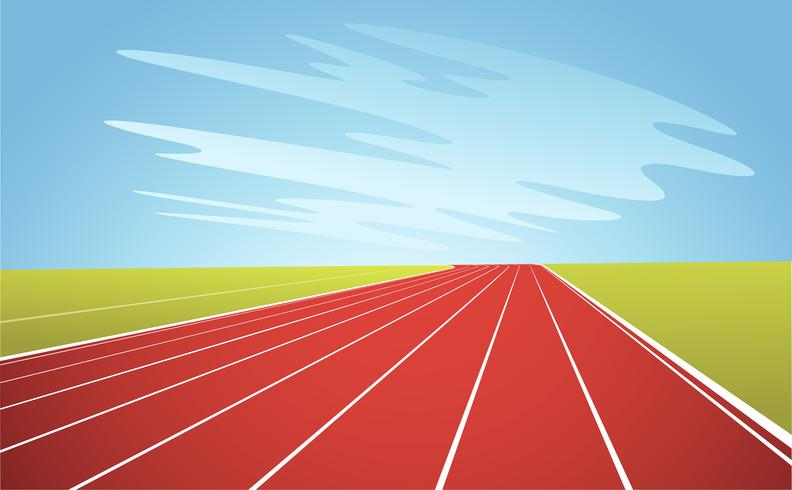
\includegraphics[width=1\textwidth]{pista}
                % \caption{Pista de corrida \cite{agostini2007}}
                \roundpic[xshift=0cm,yshift=0cm]{3.5cm}{6.5cm}{turbot_intro.png}
                %\caption{Pista de corrida \cite{agostini2007}}
            \end{figure}
        %}
        \end{center}
    \end{columns}
%*----------- notes
    \note[item]{Notes can help you to remember important information. Turn on the notes option.}
\end{frame}
%-
%*----------- SLIDE -------------------------------------------------------------
% \begin{frame}[c]{Objetivo geral} 
%     \transdissolve[duration=0.5]
   
%     \begin{center}
%         \Wider{%
%         \begin{shaded}
%         \begin{center}
%             \vspace*{0.5cm}
%             \resizebox{!}{0.7cm}{%
%               Desenvolver pesquisas em Robótica Subaquática e amadurecer a parceria com a Universidade de San Diego.
%             }%
%         \end{center}
%         \end{shaded}
%         }%
%     \end{center}
    
   
% %*----------- notes
%     \note[item]{Notes can help you to remember important information. Turn on the notes option.}
% \end{frame}
%-
%*----------- SLIDE -------------------------------------------------------------
\begin{frame}[c]{Specific goals}
  The specific goals is divided into:

  \begin{columns}[t]
    \column{.01\linewidth}
    \column{.3\linewidth}
      \begin{center}
        \begin{figure}
          \roundpic[xshift=0cm,yshift=0cm]{3.5cm}{6.5cm}{turbsim.png}
        \end{figure}
      \end{center}       
    \column{.69\linewidth}
    \begin{center}
      \begin{enumerate}
        \item Conduct SOTA on topics related to the  AUV concept; 
        \item Design the vehicle's external structure and perform CFD simulation; 
        \item Real time simulation using Gazebo and UUV Simulator \cite{7761080}; 
        \item Write papers related to the project.
      \end{enumerate}   
    \end{center}
  \end{columns}
\end{frame}
%*----------- SLIDE -------------------------------------------------------------
\begin{frame}[t]{Main requirements}
  \transboxout[duration=0.5]
  % \framesubtitle{Darwin-OP}
  \begin{columns}[c]
    \column{.5\textwidth}
      \textbf{Customer}
      \begin{itemize}
        \item Indoor/outdoor navigation
        \item Obstacle avoidance
        \item Autonomous navigation
        \item Small dimensions
        \item Energetic efficiency
        \item Emergency system
        \item Lighting system
      \end{itemize}
    \column{.5\textwidth}
      \textbf{System}
      \begin{itemize}
        \item 5 DOF and 6 thrusters composition
        \item Perceive dynamic environments
        \item 50 depth operation
        \item 1.5 m/s max velocity
        \item Max 20 kg weight
        \item 2 h of battery autonomy
        \item Positive buoyancy
      \end{itemize}
  \end{columns}
%*----------- notes
    \note[item]{Notes can help you to remember important information. Turn on the notes option.}
\end{frame}
%-

%-